\chapter{Project Budget}%
\label{app:budget}

BiasAperture is a pure-software diagnostic platform with no bill of materials or physical hardware deliverable (\cref{chap:requirements}, System Requirements); the budget below is scoped accordingly to cloud compute, subscriptions, and documentation costs rather than component procurement.

\section{Cloud Computing and Development Services}

\begin{table}[H]
    \centering
    \small
    \renewcommand{\arraystretch}{1.3}
    \caption{Cloud computing and development services cost.}%
    \label{tab:budget-cloud}
    \begin{tabular}{p{3.5cm}p{6.3cm}p{2.5cm}}
        \toprule
        \textbf{Service} & \textbf{Description} & \textbf{Cost} \\
        \midrule
        Open-source software & Python, PyTorch/TensorFlow, AIF360, Fairlearn, scikit-learn, SciPy, OpenCV, SHAP (surrogate fallback), Jinja2 & Free \\
        Cloud GPU compute (NFR-004 target) & Google Colab, free-tier T4-class GPU for full-dataset evaluation runs & Free \\
        Cloud GPU compute (contingency) & Google Colab Pro, if free-tier quota is exhausted during the full 97{,}698-image FairFace evaluation (NFR-004) & \$10/month \\
        Cloud storage & Google Drive, dataset and checkpoint storage during development & Free (existing quota) \\
        \midrule
        \multicolumn{2}{r}{\textbf{Subtotal}} & \textbf{\$0--\$10/month} \\
        \bottomrule
    \end{tabular}
\end{table}

\section{Documentation and Miscellaneous}

\begin{table}[H]
    \centering
    \small
    \renewcommand{\arraystretch}{1.3}
    \caption{Documentation and miscellaneous cost.}%
    \label{tab:budget-misc}
    \begin{tabular}{p{3.5cm}p{6.3cm}p{2.5cm}}
        \toprule
        \textbf{Category} & \textbf{Item / Description} & \textbf{Estimated Cost} \\
        \midrule
        Printing and binding & Proposal, progress, and final report copies for submission and defence & \$10--\$15 \\
        Miscellaneous & Contingency for unplanned documentation or minor tooling needs & \$5--\$10 \\
        \midrule
        \multicolumn{2}{r}{\textbf{Total Estimated Cost}} & \textbf{\$15--\$35 one-time, plus \$0--\$10/month cloud compute contingency} \\
        \bottomrule
    \end{tabular}
\end{table}

\chapter{Project Timeline}%
\label{app:timeline}

The project is executed over the eight-week schedule specified in \cref{sec:schedule}, structured into work packages WP1--WP5 as detailed in \cref{tab:wbs}. \Cref{fig:gantt-appendix} reproduces the Gantt chart of \cref{fig:gantt} for appendix reference, showing task durations, the Stream~A / Stream~B concurrency, and milestones M1--M4.

\begin{figure}[H]
    \centering
    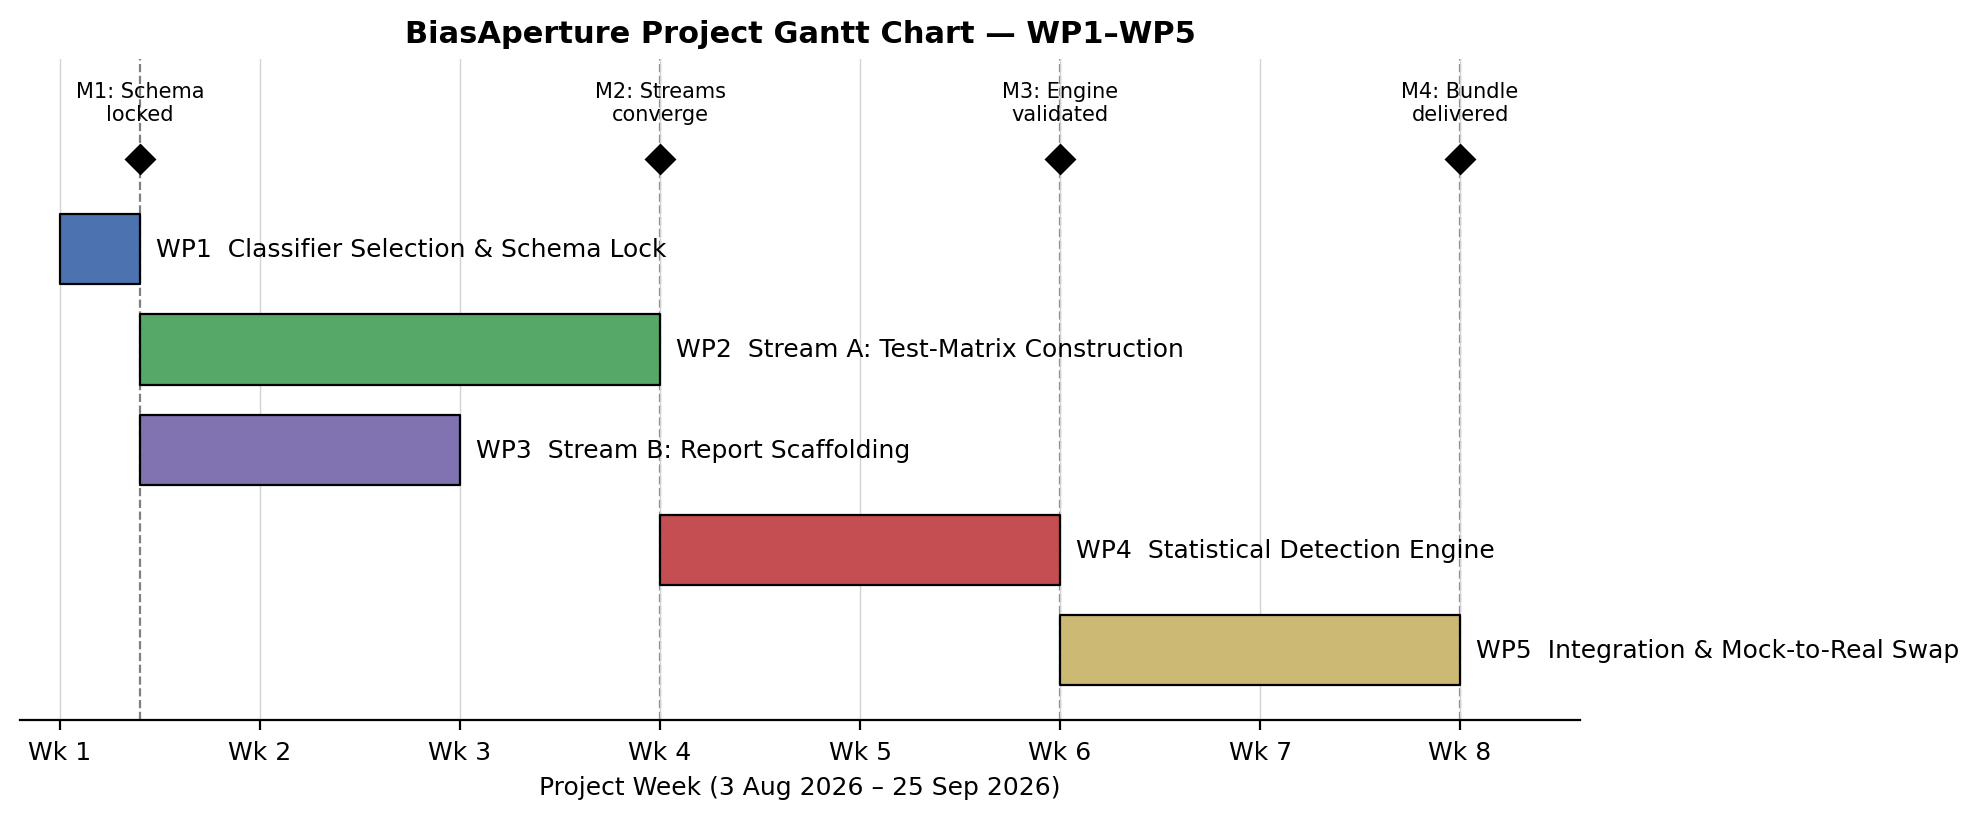
\includegraphics[width=\textwidth]{src/images/gantt.png}
    \caption{BiasAperture project schedule, work packages WP1--WP5 (reproduced from \cref{chap:methodology}).}%
    \label{fig:gantt-appendix}
\end{figure}

\chapter{Locked Internal Schema}%
\label{app:schema}

\Cref{sec:schedule} fixes the internal schema every module must honour before Stream~A and Stream~B begin parallel work. \Cref{tab:schema-testmatrix,tab:schema-metrics} give the exact field-level specification of that schema.

\begin{table}[htbp]
    \centering
    \renewcommand{\arraystretch}{1.3}
    \caption{Dataset / test-matrix schema.}%
    \label{tab:schema-testmatrix}
    \begin{tabular}{p{3.8cm}p{2.6cm}p{6.9cm}}
        \toprule
        \textbf{Field} & \textbf{Type} & \textbf{Description} \\
        \midrule
        {\ttfamily\footnotesize image\_id} & string & Unique identifier for the source image \\
        {\ttfamily\footnotesize race} & categorical (7 levels) & FairFace race / ethnicity category \\
        {\ttfamily\footnotesize gender} & categorical (binary) & Perceived gender label \\
        {\ttfamily\footnotesize age} & categorical (9 bins) & FairFace age-group bin \\
        {\ttfamily\footnotesize true\_label} & categorical & Ground-truth demographic attribute value \\
        {\ttfamily\footnotesize predicted\_label} & categorical & Value returned by the Model Interface module \\
        {\ttfamily\scriptsize protected\_attribute} & categorical & Subgroup field currently selected for disparity analysis \\
        \bottomrule
    \end{tabular}
\end{table}

\begin{table}[htbp]
    \centering
    \renewcommand{\arraystretch}{1.3}
    \caption{Metrics-dictionary schema, the shape every Fairness Metrics Computation Engine output must satisfy.}%
    \label{tab:schema-metrics}
    \begin{tabular}{p{4.3cm}p{2cm}p{6.9cm}}
        \toprule
        \textbf{Field} & \textbf{Type} & \textbf{Description} \\
        \midrule
        {\ttfamily\footnotesize metric\_name} & string & One of \gls{dpd}, \gls{eod}, \gls{eop}, \gls{dir} \\
        {\ttfamily\footnotesize subgroup\_n} & integer & Subgroup sample size \\
        {\ttfamily\footnotesize point\_estimate} & float & Computed metric value \\
        {\ttfamily\footnotesize ci\_lower}, {\ttfamily\footnotesize ci\_upper} & float pair & 95\% bootstrap confidence interval bounds ($\geq$1{,}000 resamples) \\
        {\ttfamily\footnotesize p\_value} & float & Result of the chi-squared significance test \\
        {\ttfamily\scriptsize insufficient\_sample\_flag} & boolean & True when subgroup \gls{symb:n} $< 30$ (NFR-003) \\
        \bottomrule
    \end{tabular}
\end{table}

\chapter{Risk Register}%
\label{app:riskregister}

\Cref{tab:riskregister} reproduces the risk register from the feasibility study underlying this proposal, covering the risks judged material enough to shape a design decision elsewhere in this report.

\begin{table}[htbp]
    \centering
    \renewcommand{\arraystretch}{1.3}
    \caption{Project risk register: likelihood, impact, and mitigation strategy.}%
    \label{tab:riskregister}
    \begin{tabular}{p{3cm}p{1.9cm}p{1.6cm}p{6.5cm}}
        \toprule
        \textbf{Risk} & \textbf{Likelihood} & \textbf{Impact} & \textbf{Mitigation} \\
        \midrule
        Demographic label noise, particularly UTKFace's model-estimated age labels & Medium & Medium & Formally cut UTKFace per Cut-List \#2; report subgroup \gls{symb:n} and 95\% confidence intervals alongside every metric; cross-validate against FairFace's manually annotated labels; document the limitation explicitly \\
        Model interface incompatibility with non-standard prediction formats & Medium & Medium & Provide the documented \gls{csv} / \gls{json} predictions-file ingestion path as a fallback to direct in-process inference \\
        Misinterpretation of metrics by non-specialist stakeholders & Medium & High & Plain-language explanation for every metric, with explicit caveats on statistical significance and sample size, in the generated report \\
        Scope creep toward mitigation or model retraining & Medium & High & Written scope document reviewed with the supervisor; report generation restricted to diagnostic, non-prescriptive output only \\
        Licensing non-compliance for a custom user-supplied dataset & Low & High & Display and require explicit acknowledgement of licensing terms before an audit executes (FR-009) \\
        Computational resource constraints delaying full-dataset evaluation & Low & Medium & Stratified development subset ($n=5{,}000$) supported for development; expected hardware runtimes documented (NFR-004) \\
        Dependency version drift across AIF360, Fairlearn, and the model framework & Medium & Low & Dependency versions pinned in a lock-file; periodic re-validation against upstream releases (NFR-006) \\
        Dual-use risk: findings used to exploit rather than remediate a model's weaknesses & Low & Medium & Intended, permitted use stated explicitly in project documentation; platform restricted to diagnostic reporting only \\
        \bottomrule
    \end{tabular}
\end{table}
